\documentclass[a4paper,12pt]{article}

% Packages
\usepackage[utf8]{inputenc}
\usepackage{amsmath, amssymb}
\usepackage{graphicx}
\usepackage{hyperref}
\usepackage{geometry}
\usepackage{booktabs}
\usepackage{float}
\geometry{margin=1in}

% Title Page
\title{Merit Prize Challenge 2024/2025 \\ \vspace{0.5cm} \large Breast Cancer Dataset Analysis}
\author{Guilherme José & José Caldeira}
\date{November 2024}

\begin{document}

\maketitle
\tableofcontents
\newpage

% Sections
\section{Introduction}
\label{sec:introduction}
Overview of the challenge, dataset, objectives, and methodology followed.

\subsection{Overview}
In this task, we aim to develop a model that can accurately classify a patient with or without cancer based on available medical data. This is often used to support healthcare professionals to enhance efficiency and enable doctors to help more patients effectively.
\subsection{Dataset description}
The dataset consists of \textbf{569 observations}, \textbf{30 numerical variables} and \textbf{1 binary variable}, the target. Patients are classified as having a \textbf{benign tumour} or a \textbf{malignant tumour}, the target variable is \textbf{0} or \textbf{1}, respectively. The dataset has \textbf{no missing values}.
\subsection{Critical Impact of False Negatives in Breast Cancer Prediction}
When dealing with disease forecasting, particularly dangerous types of cancer, misdiagnosing  a negative can easily be contradicted with further medical exams. The same does not happen with false negatives. When a positive patient is misdiagnosed it can lead to a false sense of security and delayed treatment. This carries a far worse consequences than a false positive. Therefore, when evaluating the models, \textbf{recall}, which represents the rate of correctly identified positive cases, should be prioritized equally or even more than accuracy.
\subsection{Logistic Regression}
Logistic regression is a machine learning method used to perform binary classification. It differs from linear regression in the activation and loss functions to update the weights. While in linear regression there is no activation function, logistic regression uses the sigmoid function:
\[ \sigma(z) = \frac{1}{1 + e^{-z}} \]


The expression of logistic regression is as follows:
\[
\hat{y} = \sigma(\mathbf{w} \cdot \mathbf{x} + b) =\frac{1}{1 + e^{-(\mathbf{w} \cdot \mathbf{x} + b)}}
\]

\begin{itemize}
    \item \(\mathbf{w}\): The weight vector.
    \item \(\mathbf{x}\): The vector with each input variable
    \item \(b\): The bias term.
    \item \(\hat{y}\): The predicted probability of the positive class (\(y=1\)). 
\end{itemize}

To evaluate the model, we use cross-validation as a loss function:
\[
\text{Loss} = -\frac{1}{N} \sum_{i=1}^{N} \left[ y_i \log(\hat{y}_i) + (1-y_i) \log(1-\hat{y}_i) \right]
\]

\subsection{EM Clustering}
The EM algorithm is an iterative technique for estimating the parameters of probabilistic models with latent variables, particularly mixtures of Gaussian distributions. Its goal is to maximize the likelihood of the observed data, given the model parameters \(\Theta = \{\pi_j, \boldsymbol{\mu}_j, \boldsymbol{\Sigma}_j\}_{j=1}^k\), where:  
\begin{itemize}
    \item \(\boldsymbol{\pi}_j\): \textit{prior} of cluster \(j\),
    \item \(\boldsymbol{\mu}_j\): mean vector of cluster \(j\),
    \item \(\boldsymbol{\Sigma}_j\): covariance matrix of cluster \(j\).
\end{itemize}

\paragraph{Steps of the EM Algorithm}
\begin{enumerate}
    \item \textbf{Initialization:} Initialize the parameters \(\Theta^{(0)}\) with some initial values.
    \item \textbf{E-step (Expectation):} Compute the \textit{posterior} \(r_{ij}\), the probability that the data point \(i\) belongs to cluster \(j\):
    \[
    r_{ij} = \frac{\pi_j^{(t)} \mathcal{N}(\mathbf{x}_i | \boldsymbol{\mu}_j^{(t)}, \boldsymbol{\Sigma}_j^{(t)})}{\sum_{l=1}^k \pi_l^{(t)} \mathcal{N}(\mathbf{x}_i | \boldsymbol{\mu}_l^{(t)}, \boldsymbol{\Sigma}_l^{(t)})},
    \]
    where \(\mathcal{N}(\mathbf{x}_i | \boldsymbol{\mu}_j, \boldsymbol{\Sigma}_j)\) is the multivariate normal density function.
    
    \item \textbf{M-step (Maximization):} Update the parameters \(\Theta\) by maximizing the expected log-likelihood:
    \[
    \pi_j^{(t+1)} = \frac{\sum_{i=1}^N r_{ij}}{N}, \quad
    \boldsymbol{\mu}_j^{(t+1)} = \frac{\sum_{i=1}^N r_{ij} \mathbf{x}_i}{\sum_{i=1}^N r_{ij}}, \quad
    \boldsymbol{\Sigma}_j^{(t+1)} = \frac{\sum_{i=1}^N r_{ij} (\mathbf{x}_i - \boldsymbol{\mu}_j^{(t+1)})(\mathbf{x}_i - \boldsymbol{\mu}_j^{(t+1)})^\top}{\sum_{i=1}^N r_{ij}}.
    \]

    \item \textbf{Convergence:} Repeat the E and M steps until the change in log-likelihood (\(\Delta \mathcal{L}\)) between iterations is below a defined threshold.
\end{enumerate}


\subsection{RBF Network}
\textbf{Radial Basis Function} is a type of neural network that uses the Radial Basis function as activation:
\[
\phi(x, c) = \exp\left(-\gamma \|x - c\|^2\right)
\]
\begin{itemize}
    \item \(\mathbf{x}\): The input vector.
    \item \(\mathbf{c}\): The centroid vector.
    \item \(\mathbf{\gamma}\): Parameter to control the width of the RBF. Also represented by \(\frac{1}{2\sigma^2}\).
\end{itemize}

RBF Networks have \textbf{3 layers}, one for the input, the middle layer, whose activation function is RBF and the output layer. The middle layer has k neurons, being \textbf{k} the \textbf{number of centroids} of the model. 

\section{Logistic Regression on the original data}
\label{sec:logistic-regression-original}
Logistic regression was applied to the raw dataset. These are the results:
\begin{itemize}
    \item \textbf{Confusion matrix}: 
    \[
    \begin{array}{|c|c|c|}
    \hline
    & \textbf{Predicted Positive} & \textbf{Predicted Negative} \\
    \hline
    \textbf{Actual Positive} & 59 & 1 \\
    \hline
    \textbf{Actual Negative} & 4 & 107 \\
    \hline
    \end{array}
    \]
    \item \textbf{Accuracy}: 97.1\%
    \item \textbf{Recall}: 93.7\%

    
\end{itemize}

The accuracy score was excellent, this might be a confirmation that the dataset is complete and easily separable for this specific problem. On the other hand, recall (percentage of actual positives that were correctly classified) was lower. This might be due to a more dispersed data in the actual positives. This should be considered, as false negatives carry a greater consequence than false positives.

\section{EM Clustering Analysis}
\label{sec:em-clustering}

\subsection{Clustering with Different \(k\) Values and Silhouette Evaluation}
EM clustering was applied to the original data with k values ranging from 2 to 10. Then we computed the silhouette metric for each of the models. These were the results:

\begin{figure}[H]
    \centering
    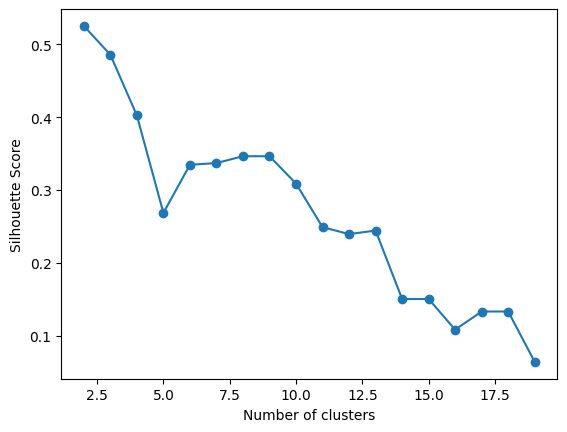
\includegraphics[width=0.5\textwidth]{imgs/silhouette.png}
    \caption{Silhoutte results across different k values.}
    \label{fig:silhouette}
\end{figure}


The results match perfectly with the nature of the problem. The more compact clusters were the ones that were binary, just like the nature of the classification tasks, which had a score of \textbf{0.63}. This confirms that the data can be easily separable, as previously mentioned in Section \ref{sec:logistic-regression-original}.

\subsection{Clustering Probabilities and Logistic Regression}
We used the previous clustering models and for each of the models, we mapped the dataset into clustering probabilities, meaning each observation is a vector of probabilities for each cluster.

Later, we used that mapped dataset to feed a logistic regression. These were the results:

\begin{figure}[H]
    \centering
    \begin{minipage}{0.48\textwidth}
        \centering
        \includegraphics[height=6cm]{imgs/accuracy_vs_k.png}  % Set a fixed height
        \caption{Accuracy results across different k values.}
        \label{fig:silhouette1}
    \end{minipage}
    \hfill
    \begin{minipage}{0.48\textwidth}
        \centering
        \includegraphics[height=6cm]{imgs/recall_vs_k.png}  % Set the same height
        \caption{Recall across different k values.}
        \label{fig:silhouette2}
    \end{minipage}
\end{figure}


The accuracy results show a slight increase from 2 to 3 in the x-axis (k values) and then decrease until k=8, after which it rises again. The first increase, even though silhouette is higher when k=2, 3 probability values might store more information than 2 and thus improve model accuracy. The decrease in accuracy is likely due to the poor silhouette score which makes the features (cluster probabilities) less informative. At the end there was a second increase in accuracy, this can be attributed to the increase in features outweight the poor silhouette scores.

The recall metric peaked when the accuracy was at its lowest, for \( k \in \{ 4, 6, 7, 8 \} \). This should be considered when choosing and evaluating models.



\section{RBF Network Training}
\label{sec:rbf-network}
We built a custom RBF Network feeding manually the \textbf{center} and \textbf{sigma} parameters. The centers were the centroids from clustering when \textbf{k = 2}, which had the highest silhouette score. Sigma was the \textbf{euclidean distance} between the 2 centroids. As for the updating of the weights, \textbf{SSE} was our loss function and \textbf{Moore-Penrose pseudoinverse} the update rule. These were the results:
\begin{itemize}
    \item \textbf{Confusion matrix}: 
    \[
    \begin{array}{|c|c|c|}
    \hline
    & \textbf{Predicted Positive} & \textbf{Predicted Negative} \\
    \hline
    \textbf{Actual Positive} & 51 & 12 \\
    \hline
    \textbf{Actual Negative} & 0 & 108 \\
    \hline
    \end{array}
    \]
    \item \textbf{Accuracy}: 93.0\%
    \item \textbf{Recall}: 81.0\%
\end{itemize}
The performance in both accuracy and recall decreased when comparing to the logistic regression in both the original and mapped dataset.  RBF Network is using the distance of the datapoints to the centers of the clusters. We can interpret each cluster center as a feature. The closer a data point is to a cluster center, the more it exhibits the characteristics of that feature. Since there are only two clusters, the model might be underfitting, as it is relying on just two features (the centroids of the clusters).

To find out if having only 2 clusters difficults learning and causes overfitting, we decided to perform RBF Network across all k values. Then we plotted the results:
\begin{figure}[H]
    \centering
    \includegraphics[width=0.5\textwidth]{imgs/rbf_vs_k.png}
    \caption{Accuracy and recall scores across different k values.}
    \label{fig:silhouette}
\end{figure}

Even though both accuracy and recall have ups and downs, overall, there is an increase in both metrics until \textbf{k = 8}, followed by a decrease in performance, likely due to overfit. These results confirm our claim that 2 clusters alone makes it hard for the model to learn the complexity of the data.

\section{Discussion}
\label{sec:discussion}
Key findings, correlations, and overall insights from the analysis.

\section{Conclusion}
\label{sec:conclusion}
Summary of the challenge, results, and future directions.

% References Section
\section*{References}
\label{sec:references}

\end{document}